% tk-01 演示题：△ABC，D 为 BC 中点；中线倍长——延长 AD 到 E 使 DE=AD，连 EC
\documentclass[tikz,border=4pt]{standalone}
\usepackage{ctex}
\usepackage{amsmath}
\usetikzlibrary{calc, decorations.markings}
\begin{document}
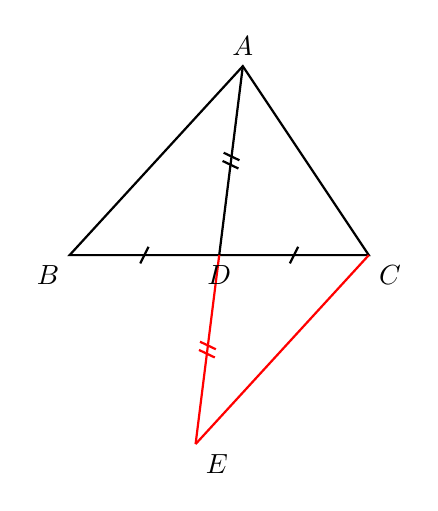
\begin{tikzpicture}[scale=1.0, thick,
  tick/.style={postaction={decorate, decoration={markings,
    mark=at position 0.5 with {\draw (-1.5pt,-3pt) -- (1.5pt,3pt);}}}},
  ticktwo/.style={postaction={decorate, decoration={markings,
    mark=at position 0.5 with {\draw (-2.5pt,-3pt) -- (-0.5pt,3pt);
                               \draw (0.5pt,-3pt)  -- (2.5pt,3pt);}}}}]
  \coordinate (A) at (0.6, 2.4);
  \coordinate (B) at (-1.6, 0);
  \coordinate (C) at (2.2, 0);
  \coordinate (D) at ($(B)!0.5!(C)$);
  % 延长 AD 至 E，DE = AD，即 E = 2D - A，相当于 A 关于 D 的对称点
  \coordinate (E) at ($(A)!2!(D)$);
  \draw (A) -- (B) -- (C) -- cycle;
  \draw[tick] (B) -- (D);
  \draw[tick] (D) -- (C);
  \draw[ticktwo] (A) -- (D);
  \draw[red, ticktwo] (D) -- (E);
  \draw[red] (E) -- (C);
  \node[above]       at (A) {$A$};
  \node[below left]  at (B) {$B$};
  \node[below right] at (C) {$C$};
  \node[below]       at (D) {$D$};
  \node[below right] at (E) {$E$};
\end{tikzpicture}
\end{document}
